\section{Experimentación}
\subsection{Mediciones y metodología de experimentación}

Para las mediciones de tiempo se tomó como base la experimentación propuesta
por la cátedra.
% Instancias:
Fueron realizadas mediciones de tiempo para la función \texttt{mstParalelo}
tomando distintas instancias de árboles, grafos ralos y completos, variando la
cantidad de nodos y cantidad de \textit{threads}.
% Repeticiones:
% se repitió 5 veces el llamado a `-e`. Dicho procedimiento usa un for
% i=0,...,9 para correrlo 10 veces obteniendo un total de 50 corridas. El
% procedimiento para correr la experimentación da 1800 filas, nuestro CSV tiene
% 9000 filas.
Debido a la naturaleza no-deterministica de la programación concurrente, se
tomaron 50 corridas para cada instancia (tipo de grafo, cantidad de nodos y
cantidad de \textit{threads}) del problema. En las
figuras~\ref{fig:arboles},~\ref{fig:ralos} y~\ref{fig:completos} se traza el
promedio y se muestra en sombreado el desvío estándar.

% CPU:
Los experimentos fueron medidos en un procesador \texttt{Intel (R) Core (TM) i5
3230M CPU @ 2.60GHz} de 2 \textit{cores} físicos y 4 \textit{cores} lógicos,
con 3072 KB de cache. En una computadora con 8 GB de memoria principal.

\subsection{Performance}

\subsubsection{Análisis Previo}
La hipótesis que sea plantea para este experimento es que la performance de la 
implementación en paralelo sea superior al secuencial. Se espera además que al 
aumentar la cantidad de nodos, la diferencia del tiempo de ejecución entre los 
algoritmos sea cada vez mayor hasta una cierta cantidad de threads.

\subsubsection{Resultados}
A partir del resultado obtenido se puede afirmar que la hipótesis planteada no 
se corresponde con el resultado empírico obtenido.
Se pudo observar que para todos los casos el tiempo de ejecución crece con el
tamaño de la instancia, tanto si su incremento es en cantidad de nodos o en
cantidad de ejes.
% Performance variando #threads
Para todas las instancias obtuvimos una mejor
\textit{performance} al ejecutar de forma secuencial, que al ejecutar más de un
\textit{thread} de forma
concurrente.
% Mas de 4 concurrente:
Puede verse que la degradación de la \textit{performance} se acentúa para las
mediciones de 8, 16 y 32 \textit{threads}, cantidad que supera la cantidad de
\textit{cores} lógicos del CPU donde fueron realizadas las mediciones.

% Acá hablo de los casos para 1,2,4 threads:
En las figuras~\ref{fig:arboles124}--\ref{fig:completos124} se muestra en
detalle el comportamiento de nuestra implementación del algoritmo para 1, 2 y 4
\textit{threads}. Puede verse que el algoritmo tiene mejor rendimiento de forma
secuencial. Para el caso de los árboles, utilizar 4 threads arrojó
mejores resultados que 2, aunque esta diferencia no es significativa.

La pérdida de rendimiento puede deberse a una mala elección o implementación
del algoritmo y las estructuras que le dan soporte. Al incrementar la 
cantidad de \textit{threads} se incrementa el tiempo en el que los mismos se
 encuentran intentando fusionarse. Las fusiones en sí involucran copiar los 
 datos de un thread al otro y reiniciar a uno de ellos. Todas estas son tareas 
 que el algoritmo secuencial no tiene que hacer. Por otro lado, la penalización
  de los cambios de contexto, inexistente en el caso secuencial, es cada vez 
  mayor a medida que crece la cantidad de threads.
  Otra diferencia entre la versión secuencial y la paralela, es que la última 
  también tiene el overhead de crear, inicializar, detener y sincronizar los 
  hilos. Si estos hilos hacen poco trabajo en relación al overhead que 
  requieren es esperable que haya una pérdida de rendimiento. Por último, 
  volvemos a señalar el hecho de que los peores resultados se obtuvieron 
  cuando la cantidad de threads seperó al número de cores lógicos de la 
  computadora donde fueron realizadas las pruebas. Si la cantidad de hilos 
  supera la cantidad de cores, no se puede lograr el paralelismo para todos 
  los hilos. La diferencia notable entre los resultados para menos de 4 threads
   y para el resto, respaldan este punto.
% FIXME tirar más hipotesis.

\newpage

\begin{figure}[h]
\caption{Mediciones para árboles.}
\centering
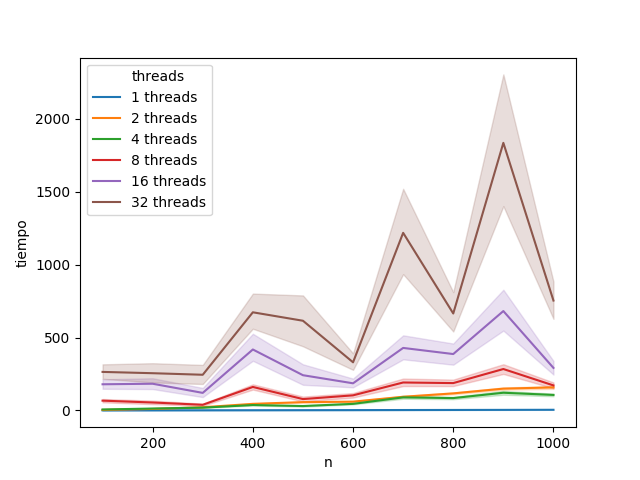
\includegraphics[width=0.4\textwidth]{imagenes/arbol.png} \\%
\label{fig:arboles}
\end{figure}

\begin{figure}[h]
\caption{Mediciones para grafos ralos.}
\centering
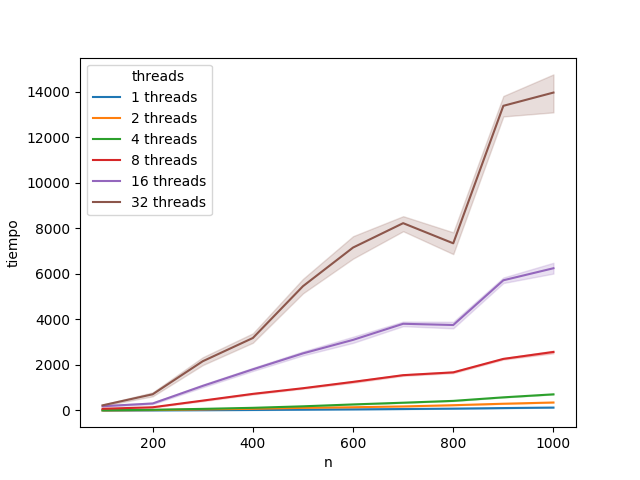
\includegraphics[width=0.4\textwidth]{imagenes/ralo.png} \\%
\label{fig:ralos}
\end{figure}

\begin{figure}[h]
\caption{Mediciones para grafos completos.}
\centering
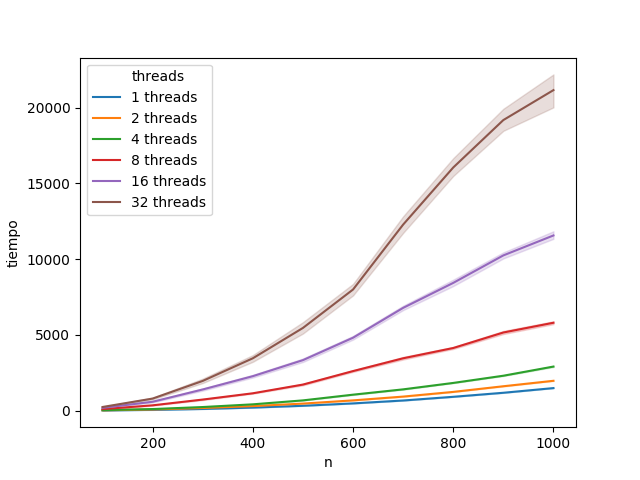
\includegraphics[width=0.4\textwidth]{imagenes/completo.png} \\%
\label{fig:completos}
\end{figure}

\newpage

\begin{figure}[h]
\caption{Mediciones para árboles con hasta 4 \textit{threads}.}
\centering
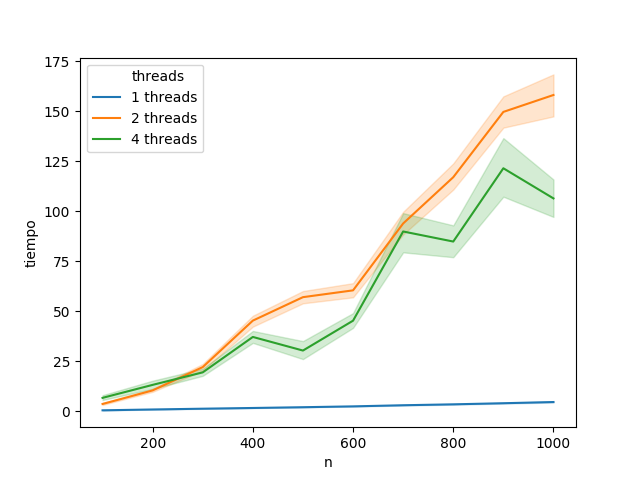
\includegraphics[width=0.4\textwidth]{imagenes/arbol-124.png} \\
\label{fig:arboles124}
\end{figure}

\begin{figure}[h]
\caption{Mediciones para grafos ralos con hasta 4 \textit{threads}.}
\centering
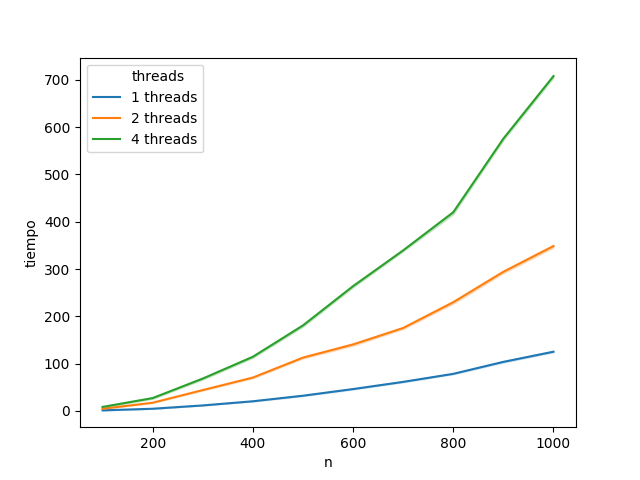
\includegraphics[width=0.4\textwidth]{imagenes/ralo-124.png} 
\label{fig:ralos124}
\end{figure}

\begin{figure}[h]
\caption{Mediciones para grafos completos con hasta 4 \textit{threads}.}
\centering
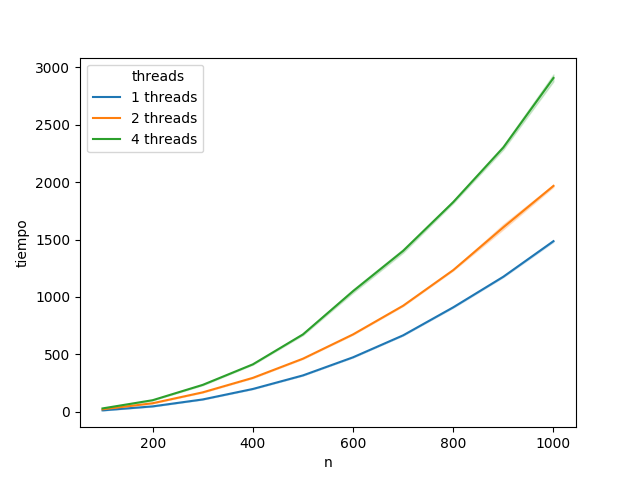
\includegraphics[width=0.4\textwidth]{imagenes/completo-124.png} \\
\label{fig:completos124}
\end{figure}

\newpage

\subsection{Fusiones}

\subsubsection{Análisis Previo}

Decidimos realizar algunas pruebas extras para los casos que menos se alejaban 
del algoritmo secuencial: o sea para los casos de 2 y 4 threads. Las pruebas 
que realizamos consistía en analizar la cantidad de intentos de fusiones y de 
fusiones efectivas para los distintos tipos de grafos (árboles, ralos y 
completos), con los distintos tamaños posibles (cantidad de nodos). La 
hipótesis es que a mayor cantidad de threads, más intentos de fusionarse 
deberíamos ver, y que este incremento también debería reflejarse en los casos 
de más nodos y más ejes.

Para realizar este experimento utilizamos un contador atómico global, al 
momento de realizar una fusión es incrementado. Usamos el mismo framework 
provisto por la cátedra con una leve modificación para imprimir este contador 
en vez del tiempo promedio. A su vez se hicieron múltiples iteraciones y se 
calculó número de fusiones promedio para graficar. Los resultados están en 
las figuras \ref{fig:fusionesarboles} a \ref{fig:fusionescompletos}.

A su vez, hicimos lo mismo para contar los intentos de fusiones, esto es, 
un contador atómico compartido por todos los hilos, que lleva la cuenta de 
la cantidad de veces que un hilo encontró que el próximo nodo a agregar había 
sido capturado por otro. Dada la naturaleza de nuestro algoritmo, este caso no 
implica necesariamente una fusión, ya que para que sea exitosa tiene que poder 
hacerse con los locks pertinentes. Los resultados están en 
las figuras \ref{fig:intentos2threads} y \ref{fig:intentos4threads}.

\subsubsection{Resultados}

Las observaciones respaldan la hipótesis como puede apreciarse en los gráficos.
 Es evidente que mientras más threads hay más fusiones hay que realizar. Se 
puede observar que el número de fusiones no crece con el mismo grado que el tamaño 
del grafo, aunque para los árboles, la cantidad de fusiones registrada fue, 
en promedio, mucho menor. Esto en parte también explica que los árboles sean 
los grafos que se resuelven en la menor cantidad de tiempo.

En cuanto a los intentos de fusión observamos que los árboles son los que menos 
intentos realizan, lo cual se relaciona con que también tengan el menor número 
de fusiones. Sin embargo, para ralos y completos quién realiza más intentos 
fue dependiente de la cantidad de threads. El hecho sobresaliente de esta 
experimentación es la diferencia en el número de intentos de fusiones entre 
las versiones de 2 y 4 threads. La diferencia es de 4 órdenes de magnitud, 
mientras que para las fusiones que efectivamente se realizan no hay ni un 
órden de magnitud entre 2 y 4 threads. Esto nos da un indicio de que la estrategia
 utilizada en nuestro algoritmo desperdicia muchos recursos en intentar lograr 
una fusión, lográndolo en una pequeña fracción de los intentos, especialmente 
a medida de que se suman threads.

\newpage

\begin{figure}[h]
   \centering
   \caption{Fusiones para árboles con hasta 4 \textit{threads}.}
   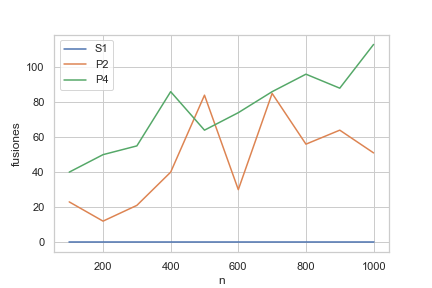
\includegraphics[width=0.45\textwidth]{imagenes/fusiones-arboles.png}
   \label{fig:fusionesarboles}
\end{figure}

\begin{figure}[h]
   \centering
   \caption{Fusiones para grafos ralos con hasta 4 \textit{threads}.}
   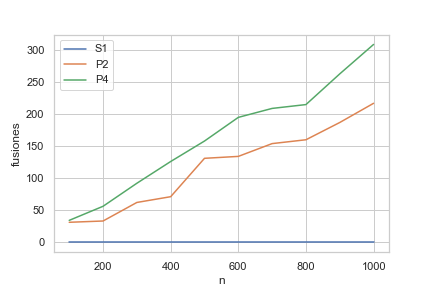
\includegraphics[width=0.45\textwidth]{imagenes/fusiones-ralos.png}
   \label{fig:fusionesralos}
\end{figure}

\begin{figure}[h]
   \centering
   \caption{Fusiones para grafos completos con hasta 4 \textit{threads}.}
   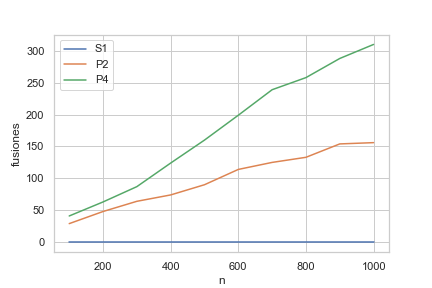
\includegraphics[width=0.45\textwidth]{imagenes/fusiones-completos.png}
   \label{fig:fusionescompletos}
\end{figure}

\newpage

\begin{figure}[h]
   \centering
   \caption{Intentos de fusiones para 2 \textit{threads}.}
   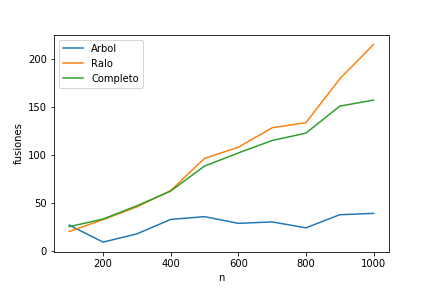
\includegraphics[width=0.5\textwidth]{imagenes/intentos-fusiones-2-threads.png}
   \label{fig:intentos2threads}
\end{figure}

\begin{figure}[h]
   \centering
   \caption{Intentos de fusiones para 4 \textit{threads}.}
   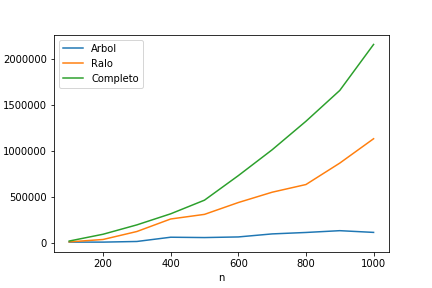
\includegraphics[width=0.5\textwidth]{imagenes/intentos-fusiones-4-threads.png}
   \label{fig:intentos4threads}
\end{figure}
